\normaltrue \difficilefalse \tdifficilefalse
\correctionfalse

%\UPSTIidClasse{11} % 11 sup, 12 spé
%\newcommand{\UPSTIidClasse}{12}
% CCP MP 2011
\exer{Système de levage à multiples colonnes $\star$ \label{A3:01:59}}
\setcounter{question}{0}\UPSTIcompetence[2]{A3-01}
\index{Compétence A3-01}
\index{Système de levage à multiples colonnes }
\index{Associer les fonctions aux constituants.}

\ifcorrection
\else
\textbf{Pas de corrigé pour cet exercice.}
\fi

\ifprof
\else

Les sociétés de transports publics des grandes agglomérations gèrent des réseaux comportant des
bus et/ou des tramways. Ces sociétés possèdent des centres de maintenance ayant en charge
l’entretien et la réparation de leurs véhicules. %Parmi ces véhicules, on peut trouver des tramways de
%deux types : sur rails ou sur pneus. 
On s'intéresse ici à la maintenance de tramways sur rails de type
TFS (Tramway Français Standard).


Le système de levage est constitué d’une armoire de commande (nommée PC) munie d’un pupitre
de commande, d’un API (Automate Programmable Industriel), de relais et cartes de commande
pour moteurs. Cette PC peut gérer jusqu’à 10 colonnes de levage. Ces colonnes de levage sont des unités indépendantes mobiles que l’on peut déplacer manuellement
grâce à des roues escamotables. Elles sont constituées d’un chariot de levage guidé par 4 galets roulant à l’intérieur d’une colonne (rails
en tôle pliée). 




L’entraînement du chariot se fait par une vis à filet trapézoïdal, mise en rotation par un moto-réducteur-frein asynchrone. On met en place les colonnes au
niveau de la plate forme du tramway à soulever, aux endroits prévus à cet effet.


%\begin{multicols}{2}
\begin{figure}[H]
\centering
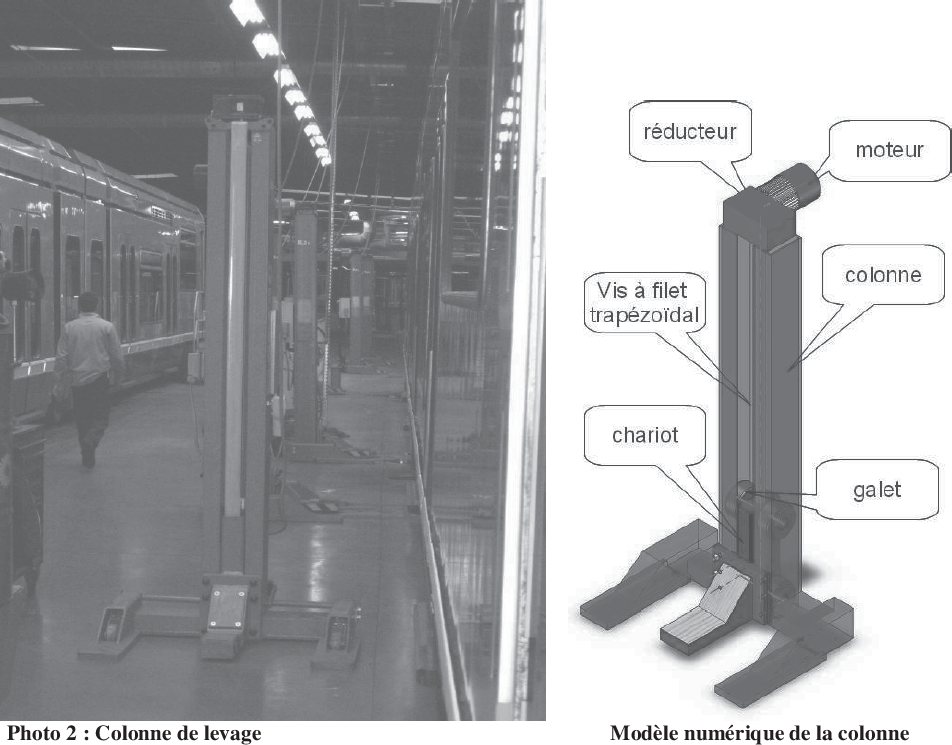
\includegraphics[height=4.5cm]{59_01}
%\caption{Amplificateur de charge à plusieurs canaux KISTLER. \label{fig_50_01}}
\end{figure}

\begin{figure}[H]
\centering
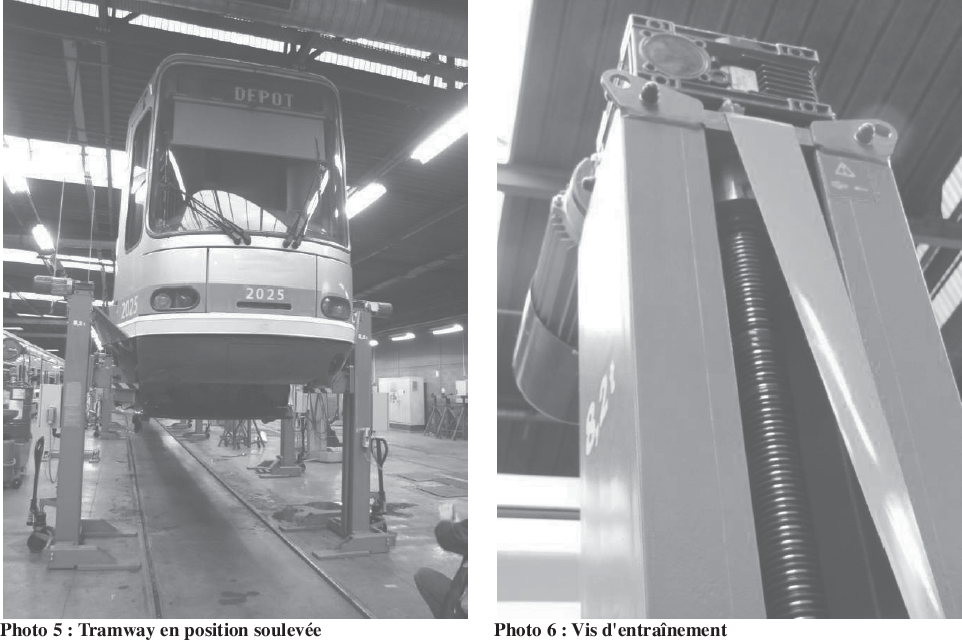
\includegraphics[height=4.5cm]{59_02}
\end{figure}

%\end{multicols}

Pour soulever un tramway de \SI{45}{tonnes} et de 30 mètres de long, le service de maintenance utilise 8
colonnes de levage d'une capacité unitaire maximale de 8,2 tonnes commandées simultanément. Lorsque les colonnes sont en place, on démarre le cycle de levage :
l’opérateur peut choisir un fonctionnement manuel ou automatique. En mode automatique, on
affiche sur le pupitre la consigne de hauteur à atteindre, la PC pilote alors chaque moteur des 8
colonnes jusqu’à ce que cette hauteur soit atteinte. Chaque colonne est équipée d’un codeur
incrémental informant la PC de la position du chariot de levage de la colonne. Pour un
fonctionnement en toute sécurité, il faut assurer une certaine horizontalité du tramway soulevé :
l'ensemble des points de levage doit être compris entre deux plans parallèles distants de \SI{20}{mm} au
maximum (coplanéité).



\begin{multicols}{2}

Le développement sous forme de FAST de la fonction principale F.P.1 (plus simplement écrite
« Soulever un tramway ») est donné ci-après.


\begin{figure}[H]
\centering
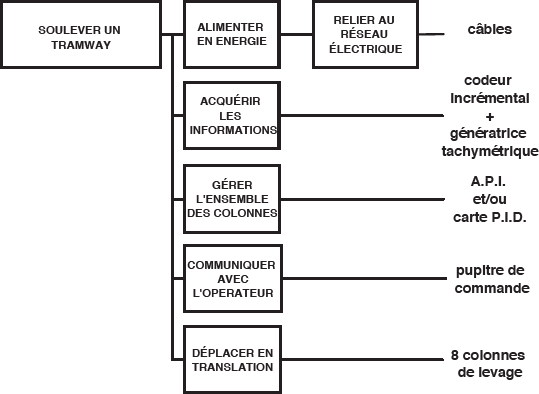
\includegraphics[height=4cm]{59_03}
\end{figure}

Le développement sous forme de FAST de la fonction technique « Déplacer en translation » pour
une colonne est donné ci-après.

\begin{figure}[H]
\centering
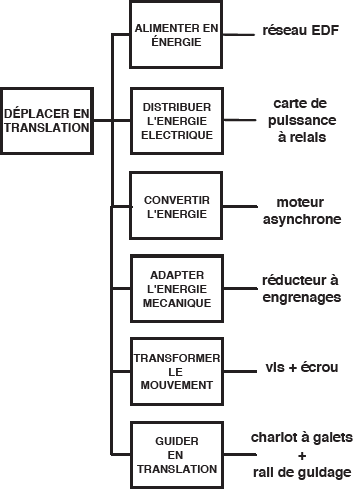
\includegraphics[height=4cm]{59_04}
\end{figure}
\end{multicols}

\fi

\question{Vous ne connaissez pas le diagramme FAST (je le sais). Quel(s) diagramme(s) SysML pourriez-vous utiliser pour remplacer les diagrammes << FAST >>.}

\question{Réaliser la chaîne fonctionnelle du système de levage étudié.}


\ifprof
\else
\begin{flushright}
\footnotesize{Corrigé  voir \ref{A3:01:59}.}
\end{flushright}%
\fi